\subsection{Selectively Inverting an Image}
\label{sect:invert}

You may be familiar with the ``invert colors'' or ``photo negative''
effect commonly available in image editors. In this problem, we will
invert the colors of only a part of an image. The part that we choose
to invert will be based on a target color and a tolerance level. You
can see an example in Figure~\ref{fig:g5_invert}.

\begin{figure}[h]
\centering
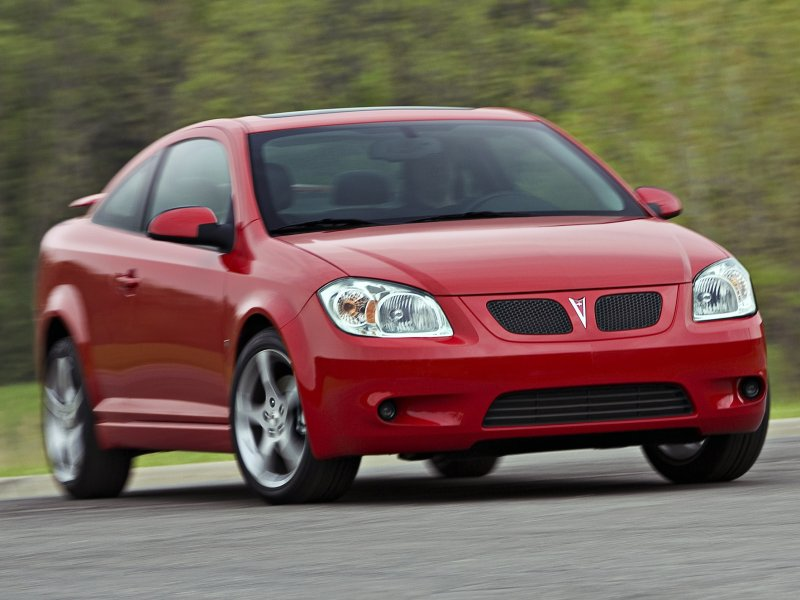
\includegraphics[scale=0.15]{\img/g5.png}
\quad
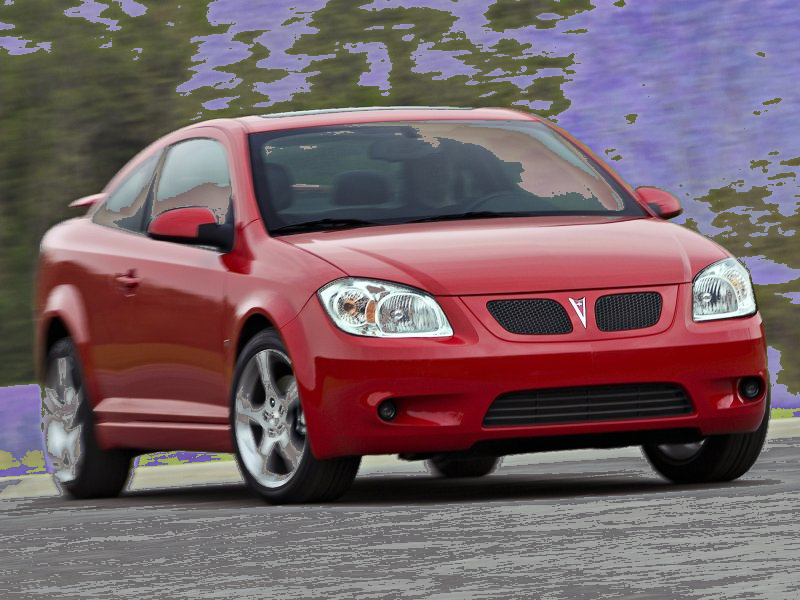
\includegraphics[scale=0.15]{\img/g5-invert1.png}
\quad
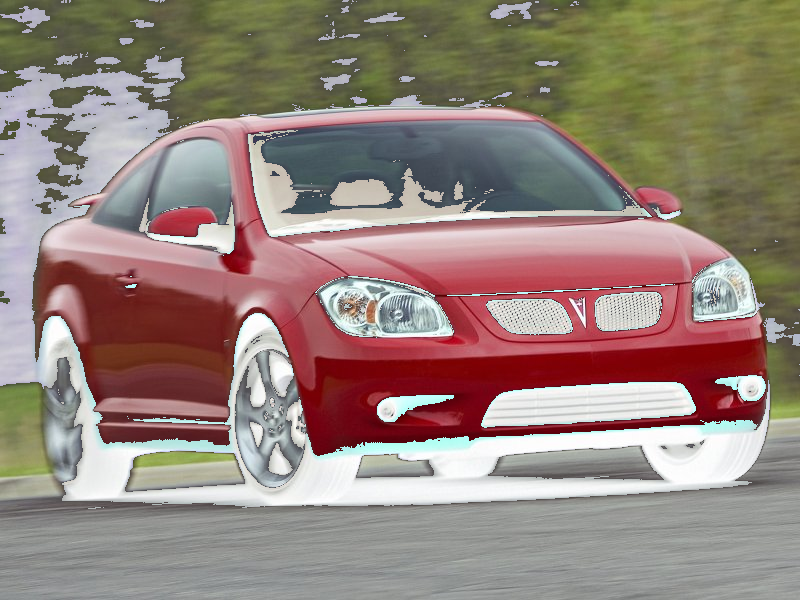
\includegraphics[scale=0.15]{\img/g5-invert2.png}
\caption{A sporty coupe with no inversion (left); partial
  inversion, color=\lstinline'0xffcf0000', tolerance=100 (middle);
  and full inversion, color=\lstinline'0xffcf0000', tolerance=255 (right).}
\label{fig:g5_invert}
\end{figure}
Given an ordinary image of size $w \times h$ along with a target color
and a tolerance, examine each pixel.  If the difference between the
starting pixel and the target color is less than or equal to the
tolerance for the red, green, and blue channels, then that pixel
should be inverted. You should not look at the alpha value.  The
tolerance will be specified as an integer between 0 and
255.  Essentially, if the target color is close enough to the color of
a particular pixel, that pixel should be inverted.  By inverting, we
mean flipping each bit. For example, suppose the color components for
a pixel are given by the bytes:

\begin{quote}
\renewcommand{\arraystretch}{1.2}
\begin{tabular}{l|lll}
   Color   & Red                  & Green                & Blue
\\\hline
   Binary  & \lstinline'01111101' & \lstinline'10100001' & \lstinline'10010111'
\\ Decimal & \lstinline'125'      & \lstinline'161'      & \lstinline'151'
\\ Hex     & \lstinline'0x7d'     & \lstinline'0xa1'     & \lstinline'0x97'
\end{tabular}
\end{quote}

And our target color is:
\begin{quote}
\renewcommand{\arraystretch}{1.2}
\begin{tabular}{l|lll}
   Color   & Red                   & Green                & Blue
\\\hline
   Decimal & \lstinline'143'       & \lstinline'178'      & \lstinline'158'
\\ Hex     & \lstinline'0x8f'      & \lstinline'0xb5'     & \lstinline'0x9e'
\end{tabular}
\end{quote}
If our tolerance is 20, then we have a match and should invert the pixel to the
following value:
\begin{quote}
\renewcommand{\arraystretch}{1.2}
\begin{tabular}{l|lll}
   Color   & Red                  & Green                & Blue
\\\hline
   Binary  & \lstinline'10000010' & \lstinline'01011110' & \lstinline'01101000'
\\ Decimal & \lstinline'130'      & \lstinline'94'       & \lstinline'104'
\\ Hex     & \lstinline'0x82'     & \lstinline'0x5e'     & \lstinline'0x68'
\end{tabular}
\end{quote}
Note that an image processed with a tolerance of 0 will only invert an exact
match and a tolerance of 255 will invert the entire image.
For each pixel, do not change its alpha component.

\vspace{0.1in}

\begin{task}[4]
\TAGS{array, correctness, safety, testing}
In the C0 file \lstinline'invert.c0', complete the \lstinline'invert'
function:
\begin{lstlisting}
pixel_t[] invert(pixel_t[] pixels, int width, int height,
                 int color, int tolerance);
\end{lstlisting}
This function should implement the algorithm described above, given an
array \lstinline'pixels' representing an image of width
\lstinline'width' and height \lstinline'height' using a target color
of \lstinline'color' and a tolerance of \lstinline'tolerance'. The
returned array should be the representation of the image after
inversion has occurred. It should \textbf{not} be destructive --- that
is, you should make your changes in a copy of the array, and not in
the original array.  You may include any auxiliary functions you need
in the same file, but you should not include a \lstinline'main()'
function. If the supplied tolerance level is out of range or if
\lstinline'width' and \lstinline'height' do not agree with the size of
the array \lstinline'pixels', your function should abort with an
annotation failure when run with the -d flag.
\end{task}

We will compile your program as follows:
\begin{lstlisting}[language={[coin]C}]
% cc0 -d imageutil.c0 invert.c0 invert-main.c0 -o invert
\end{lstlisting}
using your \lstinline'imageutil.c0' and \lstinline'invert.c0' files.
Your code must compile using these instructions with files shown in the order
given. Do NOT include a main function in your \lstinline'invert.c0' file.

After compiling, here is an example of how to call your program:
\begin{lstlisting}[language={[coin]C}]
% ./invert -i images/g5.png -o images/g5-invert.png -c 0xffcf0000 -t 100
\end{lstlisting}
Note that the target color is specified in hexadecimal, beginning with ``0x''.



%%% Local Variables:
%%% mode: latex
%%% TeX-master: "main"
%%% End:
